\documentclass[10pt,oneside,a4paper]{article}
\usepackage{amsmath,amssymb}
\usepackage{geometry}
\usepackage{multirow}
\usepackage{float}
\geometry{
 a4paper,
 total={170mm,257mm},
 left=7mm,
 right=10mm,
 top=20mm,
 } 
\usepackage{bbm}
\usepackage{amsfonts}
\usepackage{graphicx}
\usepackage{subcaption}
\usepackage{amssymb}
\usepackage{fancyhdr} 
\cfoot{\thepage}
\pagestyle{fancy} 
\fancyhf{}
\fancyhead[LE,RO]{Group 3}
\fancyhead[RE,LO]{\thepage}
\DeclareMathOperator{\E}{\mathbb{E}}



\begin{document}
\begin{flushleft}


\section{Task 1}
\subsection{}
\subsubsection{•}
Finding the first order price sensitivity of Lower Bound of Arithmetic and Geometric Asian options using likelihood ratio method. The LR formulation is given as

\begin{align*}
\mu_{C, \theta} &= \E_\theta \left(C\right) \\
& = \E_\theta\left(f \left(S\right)\right) \\
& = \int_{R^n}^{} f \left(s\right) ds\\
\mu'_{C, \theta}&= \int_{R^n}^{} f \left(s\right)\frac{d \, g_\theta\left(s\right)}{d\theta}ds\\
\end{align*}

by multiplying and dividing $g_\theta\left(s\right)$ the expectation expression is obtained

\begin{align*}
\int_{R^n}^{} f \left(s\right)\frac{d \, g_\theta\left(s\right)}{d \theta} \frac{1}{g_\theta\left(s\right) }g_\theta\left(s\right) ds &= \E_\theta \left(f\left(S\right)\frac{d \, g_\theta\left(S\right)}{d \theta} \frac{1}{g_\theta\left(S\right) }\right)\\
&= \E_\theta \left(f\left(S\right)\frac{d \,ln \, g_\theta \left(S\right)}{d \, \theta}\right)\\
\end{align*}
using the above expression, we take the expected value of the product of the discounted payoff function and the score as the LR first order sensitivity respected to $S_0$. We have the discounted payoff functions for the arithmetic Asian option Lower Bound  and for the geometric Asian option below.
\begin{align*}
LB_n &= e^{-rT}\left( \frac{1}{n}\sum_{k=1}^{n}S_k - K\right) \mathbbm{1}_{\left( \prod_{k=1}^{n}S_k\right) ^{\frac{1}{n}} >K}\\
G_n &= e^{-rT} max \left(\left(\prod_{k=1}^{n}S_k\right) ^{\frac{1}{n}} - K, 0 \right)\\
\end{align*}

the score for computing an Asian option delta is given as
\begin{align*}
\frac{d \, ln \, g_{S_{0}} (S_1, ...., S_n)}{d S_0} &= \frac{\xi\left(S_1|S_{0}\right)}{S_0 \sigma \sqrt{t_1}}\\
\end{align*}

\begin{align*}
\mu'_{LB, S_0} &= \E _{S_0}\left(e^{-rT}\left( \frac{1}{n}\sum_{k=1}^{n}S_k - K\right)\mathbbm{1}_{\left( \prod_{k=1}^{n}S_k\right) ^{\frac{1}{n} }>K} \cdot \frac{\xi\left(S_1|S_{0}\right)}{S_0 \sigma \sqrt{t_1}} \right)\\
&= \E _{S_0}\left(e^{-rT}\left( \frac{1}{n}\sum_{k=1}^{n}S_k - K\right)\mathbbm{1}_{\left( \prod_{k=1}^{n}S_k\right) ^{\frac{1}{n} }>K} \cdot \frac{ln\frac{S_1}{S_0} - \left(r - \frac{1}{2}\sigma^2\right)\left(t_1 - t_0\right)}{\sigma\sqrt{t_1 - t_0}S_0\sigma\sqrt{t_1}}\right)
\end{align*}

\vspace{5mm}

\begin{align*}
\mu'_{G, S_0} &= \E _{S_0}\left(e^{-rT}\left(\left(\prod_{k=1}^{n}S_k\right) ^{\frac{1}{n}} - K\right)^{+} \cdot \frac{\xi\left(S_i|S_{i-1}\right)}{S_0 \sigma \sqrt{t_1}} \right)\\
\end{align*}
\subsubsection{}
Now, as shown above, the lower bound payoff is discontinuous at $\left( \prod_{k=1}^{n}S_k\right) ^{\frac{1}{n}} =K$. Hence it is not possible to obtain the PW estimator. LR first order sensitivity estimator should be used instead.

\subsection{}
The exact closed formed solutions for the expected Lower Bound and the Geometric payoff are given
\begin{align*}
\E\left(LB_n\right) &= \frac{S_0 e^{-rT}}{n}\sum_{k=1}^{n} e^{\mu_k + \sigma_k^2} \cdot \mathcal{N}\left(b+a_k\right)  - K e^{-rT} \cdot \mathcal{N}\left(b \right)\\
\E\left(G_n\right) &= S_0 e^{\left(r - \frac{\sigma^2}{2} + \frac{\hat{\sigma}^2}{2}\right)\hat{T} - rT} \cdot \mathcal{N}\left(d\right) - K e^{-rT} \cdot \mathcal{N}\left(d - \hat{\sigma}\sqrt{\hat{T}}\right)
\end{align*}
by taking the derivative respected to $S_0$
\begin{align*}
\frac{d \E\left(LB_n\right)}{dS_0} &= \frac{e^{-rT}}{n}\sum_{k=1}^{n} e^{\mu_k + \sigma_k^2} \cdot \mathcal{N}\left(b+a_k\right) + \frac{S_0 e^{-rT}}{n}\sum_{k=1}^{n}e^{\mu_k + \sigma_k^2} \cdot \phi\left(b+a_k\right) \cdot \frac{1}{S_0}\frac{1}{\hat{\sigma}\sqrt{\hat{T}}}\\
& - K e^{-rT} \cdot \phi\left(b \right) \cdot \frac{1}{S_0}\frac{1}{\hat{\sigma}\sqrt{\hat{T}}}\\
 &= \frac{e^{-rT}}{n}\sum_{k=1}^{n} e^{\mu_k + \sigma_k^2} \cdot \mathcal{N}\left(b+a_k\right) + \frac{e^{-rT}}{n}\sum_{k=1}^{n}e^{\mu_k + \sigma_k^2} \cdot \phi\left(b+a_k\right) \cdot \frac{1}{\hat{\sigma}\sqrt{\hat{T}}}\\
& - K e^{-rT} \cdot \phi\left(b \right) \cdot \frac{1}{S_0}\frac{1}{\hat{\sigma}\sqrt{\hat{T}}}\\
\end{align*} 

\vspace{5mm}
\begin{align*}
\frac{d G_n}{dS_0} &= e^{\left(r - \frac{\sigma^2}{2} + \frac{\hat{\sigma}^2}{2}\right)\hat{T} - rT} \cdot \mathcal{N}\left(d\right) + S_0 e^{\left(r - \frac{\sigma^2}{2} + \frac{\hat{\sigma}^2}{2}\right)\hat{T} - rT} \phi \left(d\right) \frac{1}{S_0} \frac{1}{\hat{\sigma}\sqrt{\hat{T}}}\\
& - K e^{-rT} \cdot \phi\left(d - \hat{\sigma}\sqrt{\hat{T}}\right) \cdot \frac{1}{S_0}\frac{1}{\hat{\sigma}\sqrt{\hat{T}}}\\
&= e^{\left(r - \frac{\sigma^2}{2} + \frac{\hat{\sigma}^2}{2}\right)\hat{T} - rT} \cdot \mathcal{N}\left(d\right) +e^{\left(r - \frac{\sigma^2}{2} + \frac{\hat{\sigma}^2}{2}\right)\hat{T} - rT} \phi \left(d\right) \frac{1}{\hat{\sigma}\sqrt{\hat{T}}}\\
& - K e^{-rT} \cdot \phi\left(d - \hat{\sigma}\sqrt{\hat{T}}\right) \cdot \frac{1}{S_0}\frac{1}{\hat{\sigma}\sqrt{\hat{T}}}\\
\end{align*}

where $\mathcal{N}$ is the normal cdf and $\phi$ is the normal pdf.
\subsection{}
\subsubsection{}
Table 1 describes the computed values for the expected lower bound using different values for equally spaced dates and strike prices.

\begin{center}
\begin{table}[ht]
  \large
  \centering
  \begin{tabular}{c|c|*{4}{c|}}
    \multicolumn{5}{c}{K} \tabularnewline
    \cline{2-5}
    \multirow{6}*{\rotatebox{90}{n}} &
&    \bfseries 90 & \bfseries 100 & \bfseries 110  \tabularnewline[1 ex] 
\cline{2-5}
&    \bfseries 4 & 15.032 &  9.2449 &  5.291 \tabularnewline [1ex] 
    \cline{2-5}
&    \bfseries 12 & 14.136 &  8.2345 &  4.3702\tabularnewline [1ex] 
    \cline{2-5}
&    \bfseries 50 & 13.798 &  7.849 &  4.0268 \tabularnewline [1ex] 
    \cline{2-5}
    \cline{2-5}
  \end{tabular}
  \captionof{table}{Expected Lower Bound Values}
\end{table} 
\end{center}

Table 2 describes the computed values for the first sensitivities of the expected lower bounds using different values for equally spaced dates and strike prices.

\begin{center}
\begin{table}[ht]
  \large
  \centering
  \begin{tabular}{c|c|*{4}{c|}}
    \multicolumn{5}{c}{K} \tabularnewline
    \cline{2-5}
    \multirow{6}*{\rotatebox{90}{n}} &
&    \bfseries 90 & \bfseries 100 & \bfseries 110  \tabularnewline[1 ex] 
\cline{2-5}
&    \bfseries 4 & 0.75587 &   0.57648  &  0.39682 \tabularnewline [1ex] 
    \cline{2-5}
&    \bfseries 12 & 0.76575 &  0.56715 &  0.36875\tabularnewline [1ex] 
    \cline{2-5}
&    \bfseries 50 & 0.77045 &  0.56335 &  0.35684 \tabularnewline [1ex] 
    \cline{2-5}
    \cline{2-5}
  \end{tabular}
    \captionof{table}{Sensitivity of Expected Lower Bound Values}
\end{table} 
\end{center}


\subsubsection{}

Table 3 displays the geometric asian call option values for different n's and K's.

\begin{center}
\begin{table}[ht]
  \large
  \centering
  \begin{tabular}{c|c|*{4}{c|}}
    \multicolumn{5}{c}{K} \tabularnewline
    \cline{2-5}
    \multirow{6}*{\rotatebox{90}{n}} &
&    \bfseries 90 & \bfseries 100 & \bfseries 110  \tabularnewline[1 ex] 
\cline{2-5}
&    \bfseries 4 & 14.525 &  8.8315 &  4.971 \tabularnewline [1ex] 
    \cline{2-5}
&    \bfseries 12 & 13.602 &  7.8021 &  4.0382\tabularnewline [1ex] 
    \cline{2-5}
&    \bfseries 50 & 13.263 &  7.4155 &  3.6945 \tabularnewline [1ex] 
    \cline{2-5}
    \cline{2-5}
  \end{tabular}
\end{table} 
  \captionof{table}{Geometric Asian Call Option Values}
\end{center}

Table 4 shows the values for the first sensitivities with respect to S\textsubscript{0} for the geometric Asian option prices.

\begin{center}
\begin{table}[ht]
  \large
  \centering
  \begin{tabular}{c|c|*{4}{c|}}
    \multicolumn{5}{c}{K} \tabularnewline
    \cline{2-5}
    \multirow{6}*{\rotatebox{90}{n}} &
&    \bfseries 90 & \bfseries 100 & \bfseries 110  \tabularnewline[1 ex] 
\cline{2-5}
&    \bfseries 4 & 0.74248 &  0.56288 &  0.38356 \tabularnewline [1ex] 
    \cline{2-5}
&    \bfseries 12 & 0.75131 &  0.55277 &  0.35439\tabularnewline [1ex] 
    \cline{2-5}
&    \bfseries 50 & 0.7558 &  0.54899 &  0.34226 \tabularnewline [1ex] 
    \cline{2-5}
    \cline{2-5}
  \end{tabular}
\end{table} 
  \captionof{table}{Sensitivity of Geometric Asian Call Option Values}
\end{center}

\subsection{}
\subsubsection{}
Table 5 approximates the value of the Asian call option prices using Monte Carlo simulations and the lower bound as a control variate.  The standard error (S.E.) and the confidence intervals (C.I) can also be viewed.
\begin{center}
\begin{tabular}{|c|c|c|c|c|c|c|c|c|c|}
\multicolumn{10}{c}{K} \tabularnewline
\hline
\multirow{3}{*}{} & \multicolumn{3}{c|}{\bfseries 90}  & \multicolumn{3}{c|}{\bfseries 100} & \multicolumn{3}{c|}{\bfseries 110} \\
\cline{2-10}
 & Price & S.E. & C.I. & Price & S.E.. & C.I. & Price & S.E. & C.I \\
\hline
 \bfseries 4 & 15.0371 &  0.00020261 & 15.0367-15.0375 & 9.2492 & 0.00020476 & 9.2488-9.2496 & 5.2960 & 0.00020476 & 5.2956-5.2965   \\
\hline
 \bfseries 12 & 14.1400 & 0.00017697 & 14.1396-14.1403 & 8.2382 & 0.00017074  & 8.2379-8.2385 & 4.3749 & 0.00022525 &4.3745-4.3754 \\
\hline
 \bfseries 50 & 13.8019 & 0.00017443 & 13.8016-13.8023 & 7.8525 & 0.00014983 & 7.8522-7.8528 & 4.0315 & 0.0002129& 4.0311-4.0319 \\
  \hline
\end{tabular}
  \captionof{table}{Approximation with Lower Bound as Control Variate}
\end{center}
 
Table 6 approximates the Asian call option prices using Monte Carlo simulations and the geometric asian call option with discounted payoff as a control variate. It also includes the standard error  (S.E) and the confidence intervales (C.I.)\begin{center}
\begin{tabular}{|c|c|c|c|c|c|c|c|c|c|}
\multicolumn{10}{c}{K} \tabularnewline
\hline
\multirow{3}{*}{} & \multicolumn{3}{c|}{\bfseries 90}  & \multicolumn{3}{c|}{\bfseries 100} & \multicolumn{3}{c|}{\bfseries 110} \\
\cline{2-10}
 & Price & S.E. & C.I. & Price & S.E.. & C.I. & Price & S.E. & C.I \\
\hline
 \bfseries 4 & 15.0388 &  0.0020434 & 15.0348-15.0428 & 9.2480 & 0.0018979 & 9.2443-9.2517 & 5.2960 & 0.0018398 & 5.2924-5.2996   \\
\hline
 \bfseries 12 & 14.1386 & 0.0017756 & 14.1352-14.1421 & 8.2395 & 0.0016818  & 8.2362-8.2428 & 4.3736 & 0.0018398 &4.3706-4.3766 \\
\hline
 \bfseries 50 & 13.8030 & 0.0017397 & 13.7996-13.8064 & 7.8525 & 0.0015716 & 7.8494-7.8556 & 4.0326 & 0.0014452 & 4.0298-4.0354 \\ 
  \hline
\end{tabular}
  \captionof{table}{Approximation with Geometric Asian Call Option as Control Variate}
\end{center}

Table 7 shows the epsilon values (efficiency ratios) for the different strike prices and equally spaced dates. The values display the ratio between the two approximations with different control variates. The numerator is the efficiency of the approximation with the lower bound as a control variate and the denominator is the efficiency of the approximation with the geometric Asian option as a control variate. It is clear from Table 7 that using the expected lower bound as a control variate is more efficient than using the geometric asian call option.

\begin{center}
\begin{table}[ht]
  \large
  \centering
  \begin{tabular}{c|c|*{4}{c|}}
    \multicolumn{5}{c}{K} \tabularnewline
    \cline{2-5}
    \multirow{6}*{\rotatebox{90}{n}} &
&    \bfseries 90 & \bfseries 100 & \bfseries 110  \tabularnewline[1 ex] 
\cline{2-5}
&    \bfseries 4 & 0.0147 &  0.0162 &  0.0218 \tabularnewline [1ex] 
    \cline{2-5}
&    \bfseries 12 & 0.0120 &  0.0146 &  0.0146\tabularnewline [1ex] 
    \cline{2-5}
&    \bfseries 50 & 0.0126 &  0.0124 &  0.0236 \tabularnewline [1ex] 
    \cline{2-5}
    \cline{2-5}
  \end{tabular}
\end{table} 
  \captionof{table}{Efficiency Values for the arithmetic Asian option price}
\end{center}

\subsubsection{}
Table 8  approximates the Asian call option sensitivity with respect to S\textsubscript{0} using Monte Carlo simulations and the sensitivity of the lower bound as a control variate. The table also displays the standard errors (S.E) and the confidence intervals (C.I).
\begin{center}
\begin{tabular}{|c|c|c|c|c|c|c|c|c|c|}
\multicolumn{10}{c}{K} \tabularnewline
\hline
\multirow{3}{*}{} & \multicolumn{3}{c|}{\bfseries 90}  & \multicolumn{3}{c|}{\bfseries 100} & \multicolumn{3}{c|}{\bfseries 110} \\
\cline{2-10}
 & Price & S.E. & C.I. & Price & S.E.. & C.I. & Price & S.E. & C.I \\
\hline
 \bfseries 4 & 0.7639 &  0.00027227 & 0.7633-0.7644 & 0.5856 & 0.00029519 & 0.5850-0.5861 & 0.4071 & 0.00032565 & 0.4064-0.4077   \\
\hline
 \bfseries 12 & 0.7750 & 0.00027437 & 0.7744-0.7755 & 0.5768 & 0.00030602  & 0.5762-0.5774 & 0.3799 & 0.00033711 &0.3793-0.3806 \\
\hline
 \bfseries 50 & 0.7793 & 0.00028271 & 0.7788-0.7798 & 0.5730 & 0.00030121 & 0.5724-0.5736 & 0.3673 & 0.00033988 & 0.3667-0.3680 \\
  \hline
\end{tabular}
  \captionof{table}{Approximation with Lower Bound as Control Variate}
\end{center}
 
Table 9 approximates the Asian call option sensitivity with respect to S\textsubscript{0} using Monte Carlo simulations and the sensitivity of the geometric Asian option as a control variate. The table also displays the standard errors (S.E) and the confidence intervals (C.I).
\begin{tabular}{|c|c|c|c|c|c|c|c|c|c|}
\multicolumn{10}{c}{K} \tabularnewline
\hline
\multirow{3}{*}{} & \multicolumn{3}{c|}{\bfseries 90}  & \multicolumn{3}{c|}{\bfseries 100} & \multicolumn{3}{c|}{\bfseries 110} \\
\cline{2-10}
 & Price & S.E. & C.I. & Price & S.E.. & C.I. & Price & S.E. & C.I \\
\hline
 \bfseries 4 & 0.7560 &  0.00026752 & 0.7554-0.7565 & 0.5761 & 0.00029418 & 0.5755-0.5767 & 0.3966 & 0.00032115 & 0.3959-0.3972   \\
\hline
 \bfseries 12 & 0.7662 & 0.00028428 & 0.7656 -0.7667 & 0.5671 & 0.00030736  & 0.5664-0.5677 & 0.3686 & 0.00033728 &0.3679-0.3692 \\
\hline
 \bfseries 50 & 0.7710 & 0.00028924 & 0.7704-0.7716 & 0.5630 & 0.00030418 & 0.5624-0.5636 & 0.3577 & 0.0003561 & 0.3570-0.3584 \\ 
  \hline
\end{tabular}
  \captionof{table}{Approximation with Geometric Asian Call Option as Control Variate}

Table 10 shows the epsilon values (efficiency ratios) for the different strike prices and equally spaced dates. The values display the ratio between the two approximations with different control variates. The numerator is the efficiency of the approximation with the sensitivity  of the expected lower bound as a control variate and the denominator is the efficiency of the approximation with the sensitivity of the geometric Asian option as a control variate. It is clear from Table 10 that using the sensitivity of the expected lower bound as a control variate is more efficient than using the geometric asian call option. 
It is clear from Table 10 that the using the sensitivity of the expected lower bound is more efficient than using the geometric asian call option.
\newpage
\begin{table}[ht]
  \large
  \centering
  \begin{tabular}{c|c|*{4}{c|}}
    \multicolumn{5}{c}{K} \tabularnewline
    \cline{2-5}
    \multirow{6}*{\rotatebox{90}{n}} &
&    \bfseries 90 & \bfseries 100 & \bfseries 110  \tabularnewline[1 ex] 
\cline{2-5}
&    \bfseries 4 & 0.9858 &  0.97608 &  0.97934 \tabularnewline [1ex] 
    \cline{2-5}
&    \bfseries 12 & 0.87348 &  0.92373 &  0.95308\tabularnewline [1ex] 
    \cline{2-5}
&    \bfseries 50 & 0.90616 &  0.93272 &  0.71096 \tabularnewline [1ex] 
    \cline{2-5}
    \cline{2-5}
  \end{tabular}
    \captionof{table}{Efficiency Values for the sensitivity of the arithmetic Asian option price}
\end{table} 

\subsubsection{}
The accuracy of the 95\% confidence intervals of the control variate estimations can be displayed by the tightness that exists. This is true for all the approximations that were executed, both for the arithmetic asian call option, but also for the sensitivities. More concretely, observing tables 5,6,8 and 9 and subtracting the confidence intervals, the difference between the two values is of the 10\textsuperscript{-4} for the more accurate approximations and 10\textsuperscript{-3} for the less efficient ones. 
\newline
Control variates provide a better estimate for the estimation of the Asian Call Options and their sensitivities. In general, the higher the correlation between the variables, the more accurate the approximated value. In this case, the correlation is similar and very high between the two control variates and the payoff as well as the sensitivities, which means that the selection of the control variate is not very important.

It is also clear from the efficiency Table 7 that there is a lot more efficiency when using the lower bound as a control variate with respect to the geometric option.  Since the standard errors seem to be similar, the reason could be assigned to the construction of the control variate. 
\newline
As it is to be expected, the price of the option and of the sensitivities is more accurate the higher the n (when controlling for K). The reason for that would be that there are more values computed and a more accurate coefficient and bstarhat can be created. This is also apparent in Tables 5 and 6, where there is the standard error is less with higher n's. The downside of these is that it is more computationally expensive as more commands need to be executed. The same goes for higher K's as far as prices are concerned. 
\newline
Finally, observing Tables 1,5 and 6, it is clear that all prices are very close with the value of the expected lower bound for the price. This is to be expected, as it uses a version of the Black-Scholes formula with the Asian option payoff embedded.

\subsection{}
Running the expected lower bound with increasing values of n gives a good approximation for the precise value of the expected value. As expected the higher the value of n the better the convergence to the precise value. 


Concretely, the precise value for the expected lower bound is \textbf{7.726961356596341}. Figure 1, shows the convergence of the value with respect to increasing n's.  
\begin{figure}[H]
\centering
        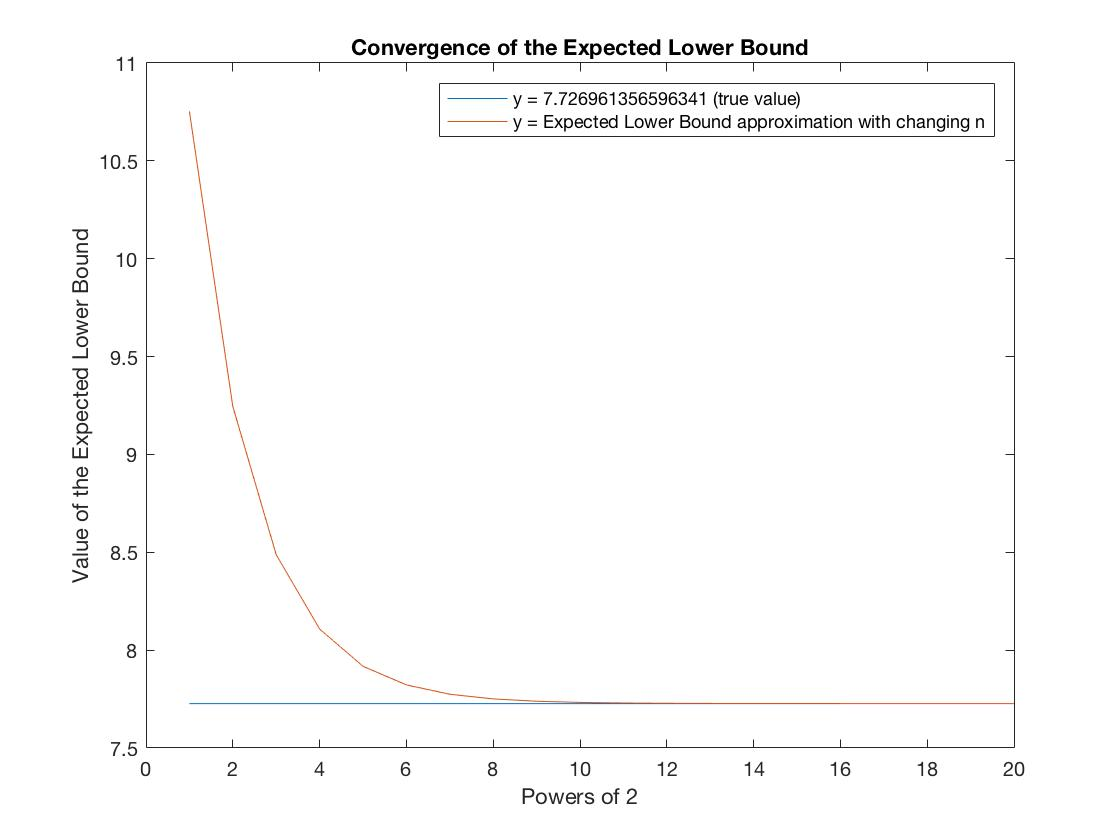
\includegraphics[totalheight=8cm]{convergence.jpg}
        \caption{Convergence of the approximation}
\end{figure}

Table SSSSSS can be reviewed for further analysis of the approximation method precision.

\begin{table}[]
\centering
\begin{tabular}{|c|c|}
\hline
\textbf{i (Power of 2)} & \textbf{Value}     \\ \hline
1                       & 10.752849553377715 \\ \hline
2                       & 9.244949514019062  \\ \hline
3                       & 8.487670434364354  \\ \hline
4                       & 8.107824667550155  \\ \hline
5                       & 7.917532175125288  \\ \hline
6                       & 7.822283197949488  \\ \hline
7                       & 7.774631600352421  \\ \hline
8                       & 7.750798836772930  \\ \hline
9                       & 7.738880689741741  \\ \hline
10                      & 7.732921171871205  \\ \hline
11                      & 7.729941301464144  \\ \hline
12                      & 7.728451338344790  \\ \hline
13                      & 7.727706349800059  \\ \hline
14                      & 7.727333853780493  \\ \hline
15                      & 7.727147605333769  \\ \hline
16                      & 7.727054481001673  \\ \hline
17                      & 7.727007918808091  \\ \hline
18                      & 7.726984637705648  \\ \hline
19                      & 7.726972997149829  \\ \hline
20                      & 7.726967176874716  \\ \hline
\end{tabular}
\captionof{table}{Approximations of the lower bound}
\end{table}
\end{flushleft}
\end{document}
